% Full-wrap KDP paperback cover (back, spine, front) for the 7 x 10 in trim, black and white interior on white paper.
% Started from templates/cover.tex of the book-writing skill, with the design of the earlier 6 x 9 in wraps.
% Spine = pages x 0.002252 in; full width = 0.125 + 7 + spine + 7 + 0.125 in; height 10.25 in (0.125 in bleed).
% Build it with the page count of the print interior, twice:
%   pdflatex "\def\InteriorPages{N}% Full-wrap KDP paperback cover (back, spine, front) for the 7 x 10 in trim, black and white interior on white paper.
% Started from templates/cover.tex of the book-writing skill, with the design of the earlier 6 x 9 in wraps.
% Spine = pages x 0.002252 in; full width = 0.125 + 7 + spine + 7 + 0.125 in; height 10.25 in (0.125 in bleed).
% Build it with the page count of the print interior, twice:
%   pdflatex "\def\InteriorPages{N}% Full-wrap KDP paperback cover (back, spine, front) for the 7 x 10 in trim, black and white interior on white paper.
% Started from templates/cover.tex of the book-writing skill, with the design of the earlier 6 x 9 in wraps.
% Spine = pages x 0.002252 in; full width = 0.125 + 7 + spine + 7 + 0.125 in; height 10.25 in (0.125 in bleed).
% Build it with the page count of the print interior, twice:
%   pdflatex "\def\InteriorPages{N}% Full-wrap KDP paperback cover (back, spine, front) for the 7 x 10 in trim, black and white interior on white paper.
% Started from templates/cover.tex of the book-writing skill, with the design of the earlier 6 x 9 in wraps.
% Spine = pages x 0.002252 in; full width = 0.125 + 7 + spine + 7 + 0.125 in; height 10.25 in (0.125 in bleed).
% Build it with the page count of the print interior, twice:
%   pdflatex "\def\InteriorPages{N}\input{cover}"
% Check it with kdp.py cover <the print interior> --cover cover.pdf (COVER OK), and cut the front cover image for
% the repository and the website with kdp.py front cover.pdf --out ../../pdf/cover.jpg.
% KDP prints spine text only on books of more than 79 pages. Everything but the art stays 0.375 in inside the trim.
\providecommand\InteriorPages{311}
\documentclass{article}
\usepackage{tikz,graphicx,xcolor}
\graphicspath{{../figures/}}
\pgfmathsetmacro\Spine{\InteriorPages*0.002252}
\pgfmathsetmacro\W{14.25+\Spine}
\pgfmathsetmacro\FrontL{7.125+\Spine}
\pgfmathsetmacro\FrontC{\FrontL+3.5}
\pgfmathsetmacro\SpineC{7.125+\Spine/2}
\pgfmathsetmacro\SpineFont{min(14,(\Spine-0.125)*72*0.8)}
\usepackage[paperwidth=\W in,paperheight=10.25in,margin=0in]{geometry}
\usepackage[T1]{fontenc}
\usepackage[sc]{mathpazo}
\definecolor{ground}{HTML}{0B0A1A}
\definecolor{accent}{HTML}{F2A541}
\definecolor{ink}{HTML}{F4EDE4}
\pagestyle{empty}
\begin{document}
\noindent\begin{tikzpicture}[x=1in,y=1in,remember picture,overlay,shift={(current page.south west)}]
\fill[ground] (0,0) rectangle (\W,10.25);
% front: the coral of art_cover.py, clipped to the front panel and its bleed
\begin{scope}
\clip (\FrontL,0) rectangle (\W,10.25);
\node[inner sep=0] at (\FrontL+3.5625,5.125) {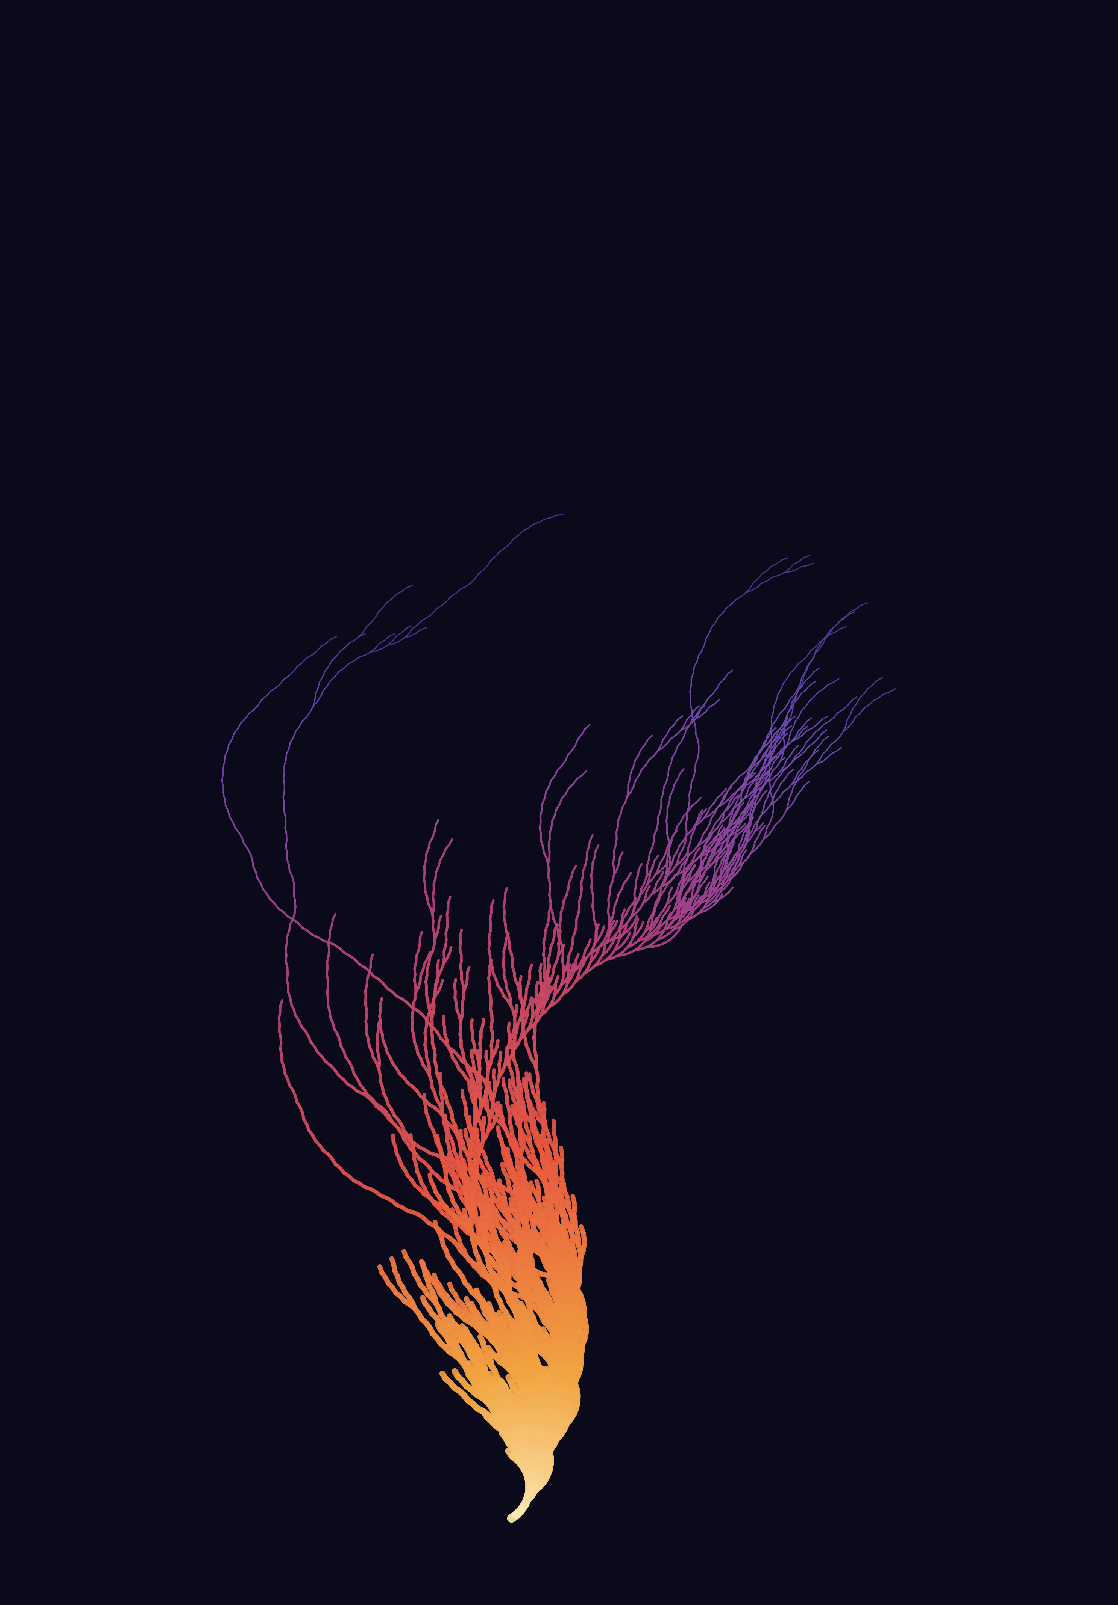
\includegraphics[width=7.25in]{art_cover}};
\end{scope}
\node[text=ink,align=center,text width=6.2in,anchor=north] at (\FrontC,9.3) {\fontsize{31}{37}\selectfont\scshape\mbox{On\hspace{0.32em}the\hspace{0.32em}Collatz\hspace{0.32em}Conjecture}};
\node[text=accent,align=center,text width=6.2in,anchor=north] at (\FrontC,8.35) {\fontsize{17}{21}\selectfont\itshape Martingales, Momentum and Continued Fractions};
\node[text=ink,align=center,text width=6.2in,anchor=north] at (\FrontC,7.75) {\fontsize{17}{21}\selectfont Nick Polson\qquad Vadim Sokolov};
% spine
\ifnum\InteriorPages>79
\node[text=ink,rotate=-90,anchor=center] at (\SpineC,6.6) {\fontsize{\SpineFont}{\SpineFont}\selectfont\scshape On the Collatz Conjecture};
\node[text=accent,rotate=-90,anchor=center] at (\SpineC,1.9) {\fontsize{\SpineFont}{\SpineFont}\selectfont\scshape Polson\enspace\textperiodcentered\enspace Sokolov};
\fi
% back
\node[text=ink,anchor=north west,text width=5.5in,align=left,inner sep=0] at (0.8,9.4) {%
\fontsize{11.25}{15.2}\selectfont\hyphenpenalty=10000\exhyphenpenalty=10000
{\color{accent}\fontsize{13.5}{17.5}\selectfont\itshape Take a positive integer. If it is even, halve it; if it is odd, triple it and add one. Repeat.\par}
\medskip
The Collatz conjecture says that every starting value eventually reaches $1$. It can be explained to a child in a minute and has resisted every attempt at proof since the 1930s. This book is about why.\par\smallskip
Reading the map as a random walk, an optimizer and a Diophantine problem, the authors split the conjecture into a divergence half, a law of large numbers for a single deterministic orbit, and a cycle half, a question about rational approximation of $\log_23$ that Diophantine information alone cannot finish. Along the way they prove that no Lyapunov function increasing in the number certifies descent over any fixed number of steps and that no finite residue sieve certifies descent for every integer, and they set out a computational path to the problem with its limits made precise.\par\smallskip
The arithmetic of the map also yields an algorithm. Switching MM, a first order method with momentum $\log_23-1$ applied on alternate steps, has an explicit linear rate at step $1/L$ on smooth strongly convex functions, and on quadratics with additive gradient noise, at steps up to $1/L$, its noise variance stays below $5/3$ times that of gradient descent for every momentum coefficient below one.\par\smallskip
With full proofs, open problems and code for every number, this is a book for probabilists, number theorists and optimizers alike.\par\bigskip
{\color{accent}\itshape Nick Polson} is the Robert Law, Jr.\ Professor of Econometrics and Statistics at the University of Chicago Booth School of Business. {\color{accent}\itshape Vadim Sokolov} is a faculty member in the Department of Systems Engineering and Operations Research at George Mason University.\par};
\node[anchor=south west,inner sep=0] at (0.8,0.6) {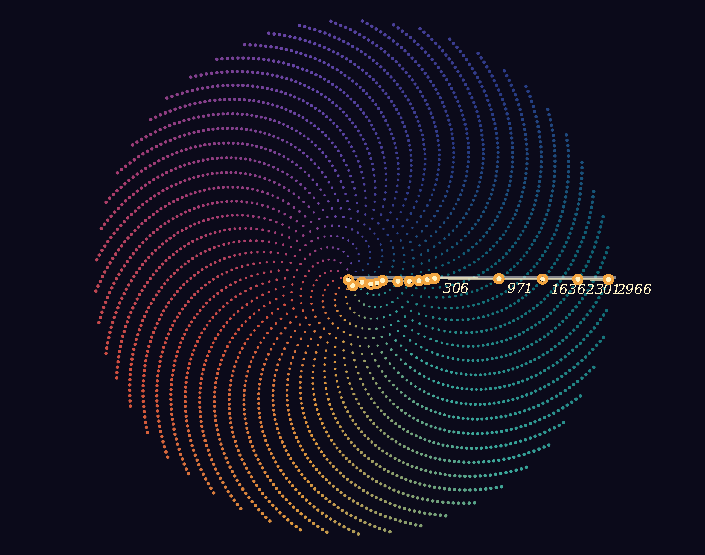
\includegraphics[width=1.9in]{art_part3}};
% barcode area, kept clear: KDP prints the barcode here
\fill[white] (4.875,0.375) rectangle (6.875,1.575);
\end{tikzpicture}
\end{document}
"
% Check it with kdp.py cover <the print interior> --cover cover.pdf (COVER OK), and cut the front cover image for
% the repository and the website with kdp.py front cover.pdf --out ../../pdf/cover.jpg.
% KDP prints spine text only on books of more than 79 pages. Everything but the art stays 0.375 in inside the trim.
\providecommand\InteriorPages{311}
\documentclass{article}
\usepackage{tikz,graphicx,xcolor}
\graphicspath{{../figures/}}
\pgfmathsetmacro\Spine{\InteriorPages*0.002252}
\pgfmathsetmacro\W{14.25+\Spine}
\pgfmathsetmacro\FrontL{7.125+\Spine}
\pgfmathsetmacro\FrontC{\FrontL+3.5}
\pgfmathsetmacro\SpineC{7.125+\Spine/2}
\pgfmathsetmacro\SpineFont{min(14,(\Spine-0.125)*72*0.8)}
\usepackage[paperwidth=\W in,paperheight=10.25in,margin=0in]{geometry}
\usepackage[T1]{fontenc}
\usepackage[sc]{mathpazo}
\definecolor{ground}{HTML}{0B0A1A}
\definecolor{accent}{HTML}{F2A541}
\definecolor{ink}{HTML}{F4EDE4}
\pagestyle{empty}
\begin{document}
\noindent\begin{tikzpicture}[x=1in,y=1in,remember picture,overlay,shift={(current page.south west)}]
\fill[ground] (0,0) rectangle (\W,10.25);
% front: the coral of art_cover.py, clipped to the front panel and its bleed
\begin{scope}
\clip (\FrontL,0) rectangle (\W,10.25);
\node[inner sep=0] at (\FrontL+3.5625,5.125) {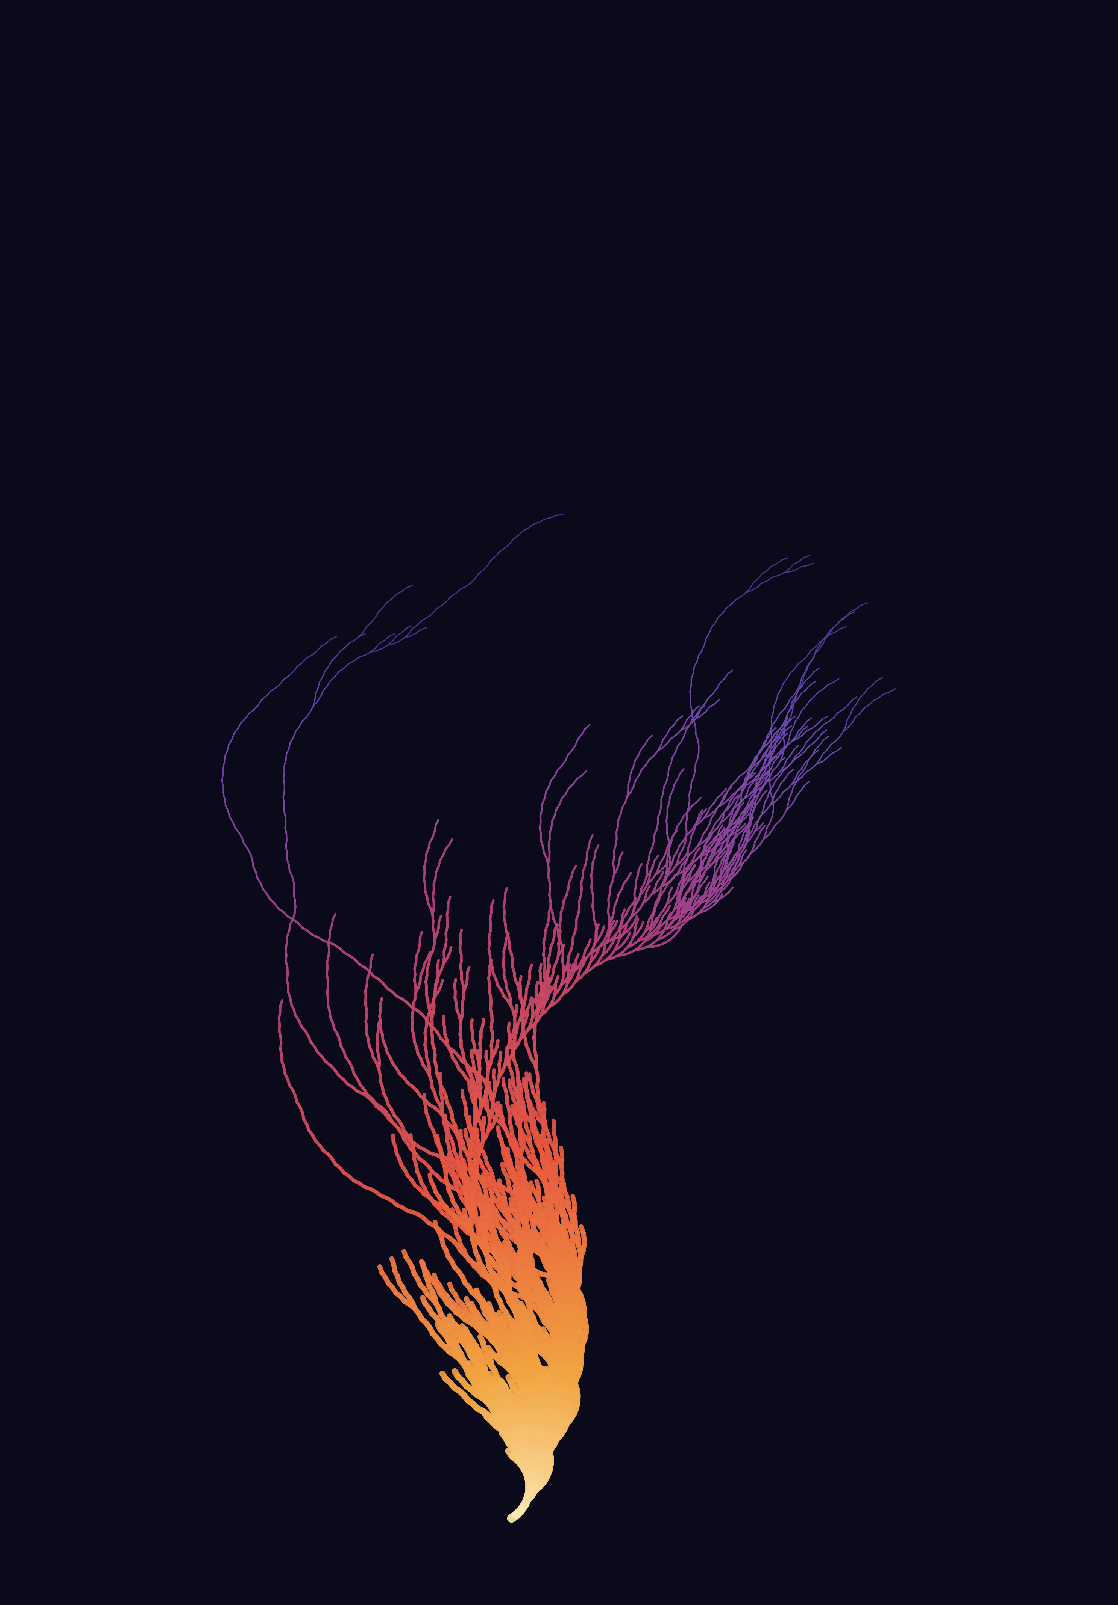
\includegraphics[width=7.25in]{art_cover}};
\end{scope}
\node[text=ink,align=center,text width=6.2in,anchor=north] at (\FrontC,9.3) {\fontsize{31}{37}\selectfont\scshape\mbox{On\hspace{0.32em}the\hspace{0.32em}Collatz\hspace{0.32em}Conjecture}};
\node[text=accent,align=center,text width=6.2in,anchor=north] at (\FrontC,8.35) {\fontsize{17}{21}\selectfont\itshape Martingales, Momentum and Continued Fractions};
\node[text=ink,align=center,text width=6.2in,anchor=north] at (\FrontC,7.75) {\fontsize{17}{21}\selectfont Nick Polson\qquad Vadim Sokolov};
% spine
\ifnum\InteriorPages>79
\node[text=ink,rotate=-90,anchor=center] at (\SpineC,6.6) {\fontsize{\SpineFont}{\SpineFont}\selectfont\scshape On the Collatz Conjecture};
\node[text=accent,rotate=-90,anchor=center] at (\SpineC,1.9) {\fontsize{\SpineFont}{\SpineFont}\selectfont\scshape Polson\enspace\textperiodcentered\enspace Sokolov};
\fi
% back
\node[text=ink,anchor=north west,text width=5.5in,align=left,inner sep=0] at (0.8,9.4) {%
\fontsize{11.25}{15.2}\selectfont\hyphenpenalty=10000\exhyphenpenalty=10000
{\color{accent}\fontsize{13.5}{17.5}\selectfont\itshape Take a positive integer. If it is even, halve it; if it is odd, triple it and add one. Repeat.\par}
\medskip
The Collatz conjecture says that every starting value eventually reaches $1$. It can be explained to a child in a minute and has resisted every attempt at proof since the 1930s. This book is about why.\par\smallskip
Reading the map as a random walk, an optimizer and a Diophantine problem, the authors split the conjecture into a divergence half, a law of large numbers for a single deterministic orbit, and a cycle half, a question about rational approximation of $\log_23$ that Diophantine information alone cannot finish. Along the way they prove that no Lyapunov function increasing in the number certifies descent over any fixed number of steps and that no finite residue sieve certifies descent for every integer, and they set out a computational path to the problem with its limits made precise.\par\smallskip
The arithmetic of the map also yields an algorithm. Switching MM, a first order method with momentum $\log_23-1$ applied on alternate steps, has an explicit linear rate at step $1/L$ on smooth strongly convex functions, and on quadratics with additive gradient noise, at steps up to $1/L$, its noise variance stays below $5/3$ times that of gradient descent for every momentum coefficient below one.\par\smallskip
With full proofs, open problems and code for every number, this is a book for probabilists, number theorists and optimizers alike.\par\bigskip
{\color{accent}\itshape Nick Polson} is the Robert Law, Jr.\ Professor of Econometrics and Statistics at the University of Chicago Booth School of Business. {\color{accent}\itshape Vadim Sokolov} is a faculty member in the Department of Systems Engineering and Operations Research at George Mason University.\par};
\node[anchor=south west,inner sep=0] at (0.8,0.6) {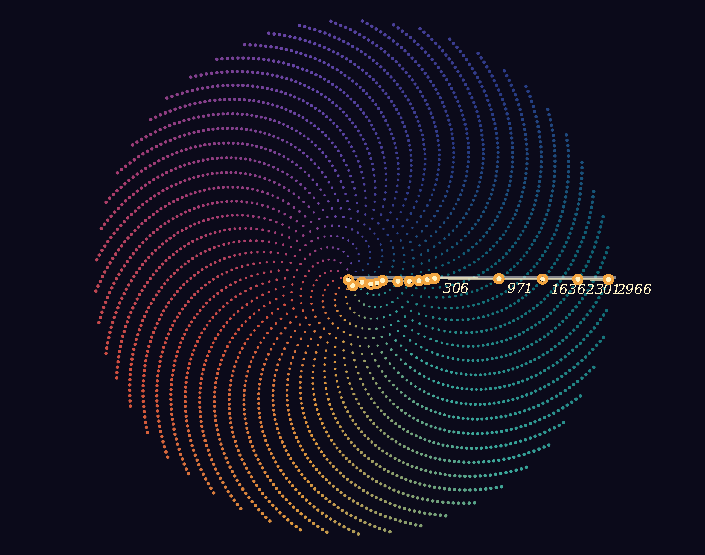
\includegraphics[width=1.9in]{art_part3}};
% barcode area, kept clear: KDP prints the barcode here
\fill[white] (4.875,0.375) rectangle (6.875,1.575);
\end{tikzpicture}
\end{document}
"
% Check it with kdp.py cover <the print interior> --cover cover.pdf (COVER OK), and cut the front cover image for
% the repository and the website with kdp.py front cover.pdf --out ../../pdf/cover.jpg.
% KDP prints spine text only on books of more than 79 pages. Everything but the art stays 0.375 in inside the trim.
\providecommand\InteriorPages{311}
\documentclass{article}
\usepackage{tikz,graphicx,xcolor}
\graphicspath{{../figures/}}
\pgfmathsetmacro\Spine{\InteriorPages*0.002252}
\pgfmathsetmacro\W{14.25+\Spine}
\pgfmathsetmacro\FrontL{7.125+\Spine}
\pgfmathsetmacro\FrontC{\FrontL+3.5}
\pgfmathsetmacro\SpineC{7.125+\Spine/2}
\pgfmathsetmacro\SpineFont{min(14,(\Spine-0.125)*72*0.8)}
\usepackage[paperwidth=\W in,paperheight=10.25in,margin=0in]{geometry}
\usepackage[T1]{fontenc}
\usepackage[sc]{mathpazo}
\definecolor{ground}{HTML}{0B0A1A}
\definecolor{accent}{HTML}{F2A541}
\definecolor{ink}{HTML}{F4EDE4}
\pagestyle{empty}
\begin{document}
\noindent\begin{tikzpicture}[x=1in,y=1in,remember picture,overlay,shift={(current page.south west)}]
\fill[ground] (0,0) rectangle (\W,10.25);
% front: the coral of art_cover.py, clipped to the front panel and its bleed
\begin{scope}
\clip (\FrontL,0) rectangle (\W,10.25);
\node[inner sep=0] at (\FrontL+3.5625,5.125) {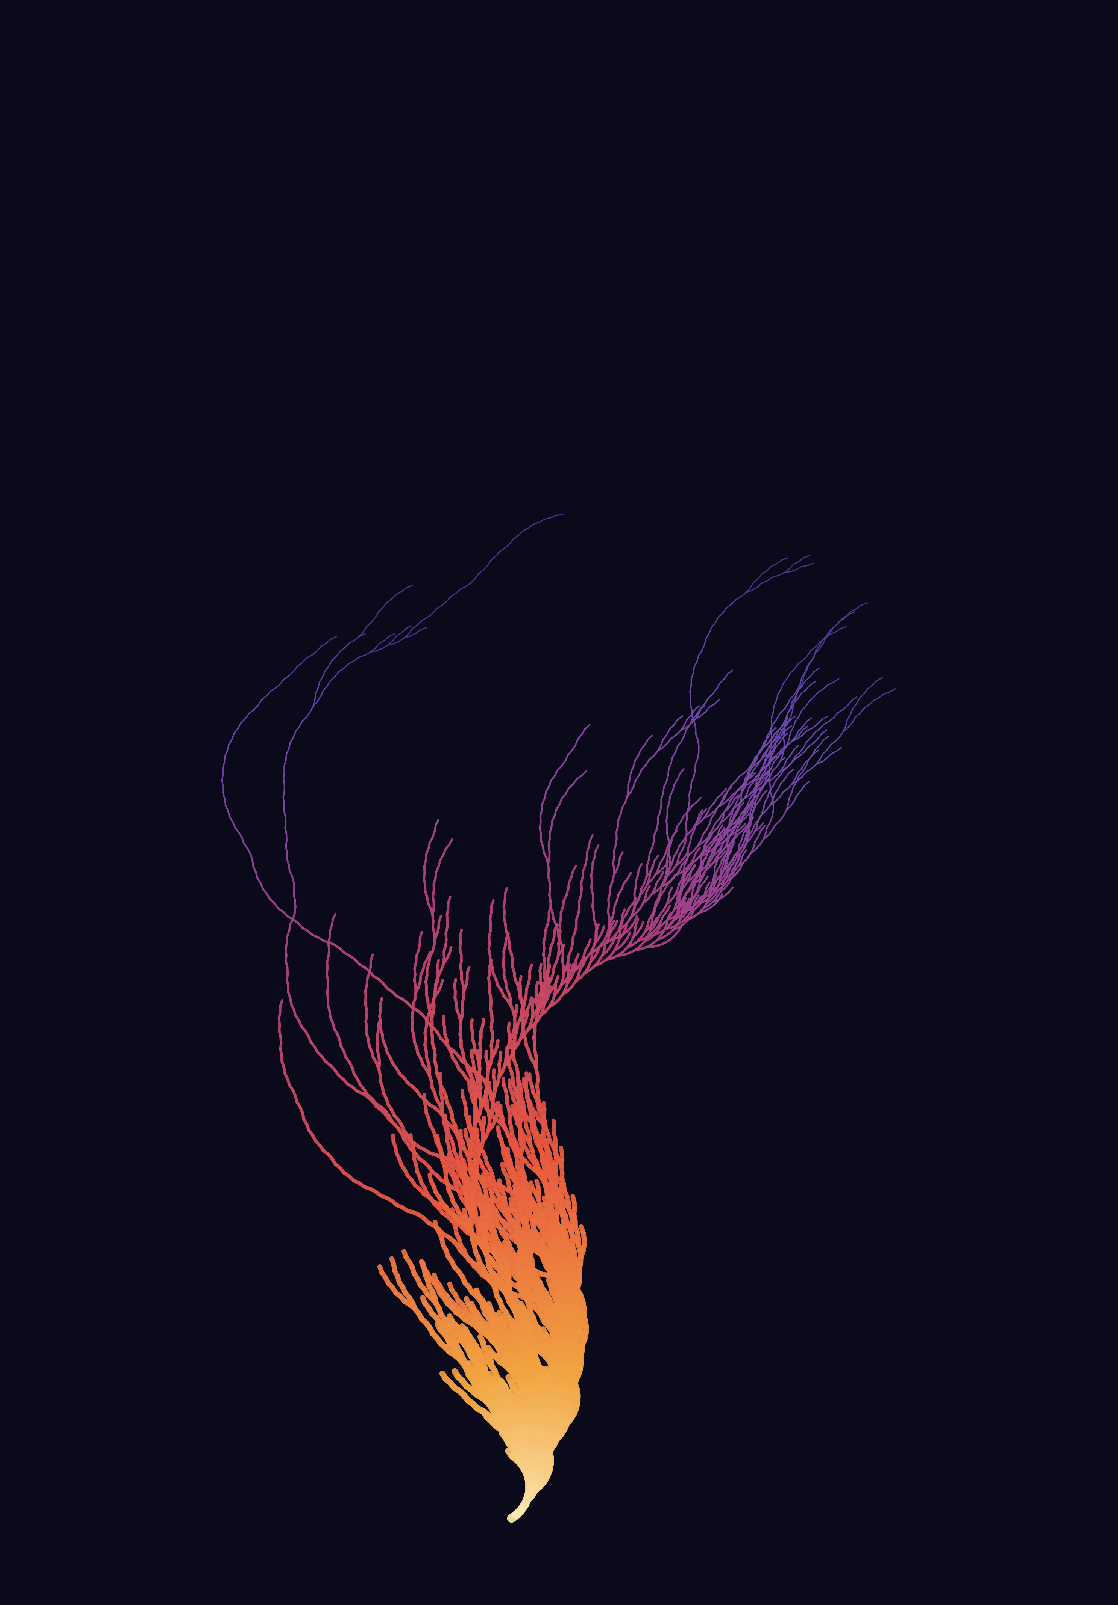
\includegraphics[width=7.25in]{art_cover}};
\end{scope}
\node[text=ink,align=center,text width=6.2in,anchor=north] at (\FrontC,9.3) {\fontsize{31}{37}\selectfont\scshape\mbox{On\hspace{0.32em}the\hspace{0.32em}Collatz\hspace{0.32em}Conjecture}};
\node[text=accent,align=center,text width=6.2in,anchor=north] at (\FrontC,8.35) {\fontsize{17}{21}\selectfont\itshape Martingales, Momentum and Continued Fractions};
\node[text=ink,align=center,text width=6.2in,anchor=north] at (\FrontC,7.75) {\fontsize{17}{21}\selectfont Nick Polson\qquad Vadim Sokolov};
% spine
\ifnum\InteriorPages>79
\node[text=ink,rotate=-90,anchor=center] at (\SpineC,6.6) {\fontsize{\SpineFont}{\SpineFont}\selectfont\scshape On the Collatz Conjecture};
\node[text=accent,rotate=-90,anchor=center] at (\SpineC,1.9) {\fontsize{\SpineFont}{\SpineFont}\selectfont\scshape Polson\enspace\textperiodcentered\enspace Sokolov};
\fi
% back
\node[text=ink,anchor=north west,text width=5.5in,align=left,inner sep=0] at (0.8,9.4) {%
\fontsize{11.25}{15.2}\selectfont\hyphenpenalty=10000\exhyphenpenalty=10000
{\color{accent}\fontsize{13.5}{17.5}\selectfont\itshape Take a positive integer. If it is even, halve it; if it is odd, triple it and add one. Repeat.\par}
\medskip
The Collatz conjecture says that every starting value eventually reaches $1$. It can be explained to a child in a minute and has resisted every attempt at proof since the 1930s. This book is about why.\par\smallskip
Reading the map as a random walk, an optimizer and a Diophantine problem, the authors split the conjecture into a divergence half, a law of large numbers for a single deterministic orbit, and a cycle half, a question about rational approximation of $\log_23$ that Diophantine information alone cannot finish. Along the way they prove that no Lyapunov function increasing in the number certifies descent over any fixed number of steps and that no finite residue sieve certifies descent for every integer, and they set out a computational path to the problem with its limits made precise.\par\smallskip
The arithmetic of the map also yields an algorithm. Switching MM, a first order method with momentum $\log_23-1$ applied on alternate steps, has an explicit linear rate at step $1/L$ on smooth strongly convex functions, and on quadratics with additive gradient noise, at steps up to $1/L$, its noise variance stays below $5/3$ times that of gradient descent for every momentum coefficient below one.\par\smallskip
With full proofs, open problems and code for every number, this is a book for probabilists, number theorists and optimizers alike.\par\bigskip
{\color{accent}\itshape Nick Polson} is the Robert Law, Jr.\ Professor of Econometrics and Statistics at the University of Chicago Booth School of Business. {\color{accent}\itshape Vadim Sokolov} is a faculty member in the Department of Systems Engineering and Operations Research at George Mason University.\par};
\node[anchor=south west,inner sep=0] at (0.8,0.6) {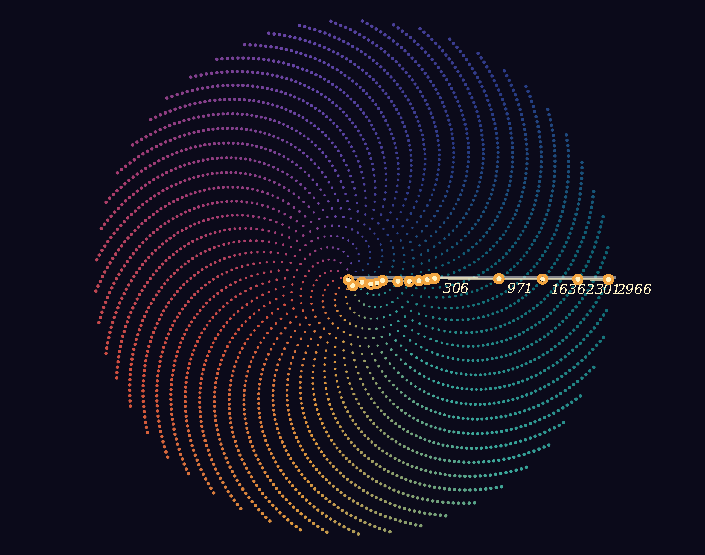
\includegraphics[width=1.9in]{art_part3}};
% barcode area, kept clear: KDP prints the barcode here
\fill[white] (4.875,0.375) rectangle (6.875,1.575);
\end{tikzpicture}
\end{document}
"
% Check it with kdp.py cover <the print interior> --cover cover.pdf (COVER OK), and cut the front cover image for
% the repository and the website with kdp.py front cover.pdf --out ../../pdf/cover.jpg.
% KDP prints spine text only on books of more than 79 pages. Everything but the art stays 0.375 in inside the trim.
\providecommand\InteriorPages{311}
\documentclass{article}
\usepackage{tikz,graphicx,xcolor}
\graphicspath{{../figures/}}
\pgfmathsetmacro\Spine{\InteriorPages*0.002252}
\pgfmathsetmacro\W{14.25+\Spine}
\pgfmathsetmacro\FrontL{7.125+\Spine}
\pgfmathsetmacro\FrontC{\FrontL+3.5}
\pgfmathsetmacro\SpineC{7.125+\Spine/2}
\pgfmathsetmacro\SpineFont{min(14,(\Spine-0.125)*72*0.8)}
\usepackage[paperwidth=\W in,paperheight=10.25in,margin=0in]{geometry}
\usepackage[T1]{fontenc}
\usepackage[sc]{mathpazo}
\definecolor{ground}{HTML}{0B0A1A}
\definecolor{accent}{HTML}{F2A541}
\definecolor{ink}{HTML}{F4EDE4}
\pagestyle{empty}
\begin{document}
\noindent\begin{tikzpicture}[x=1in,y=1in,remember picture,overlay,shift={(current page.south west)}]
\fill[ground] (0,0) rectangle (\W,10.25);
% front: the coral of art_cover.py, clipped to the front panel and its bleed
\begin{scope}
\clip (\FrontL,0) rectangle (\W,10.25);
\node[inner sep=0] at (\FrontL+3.5625,5.125) {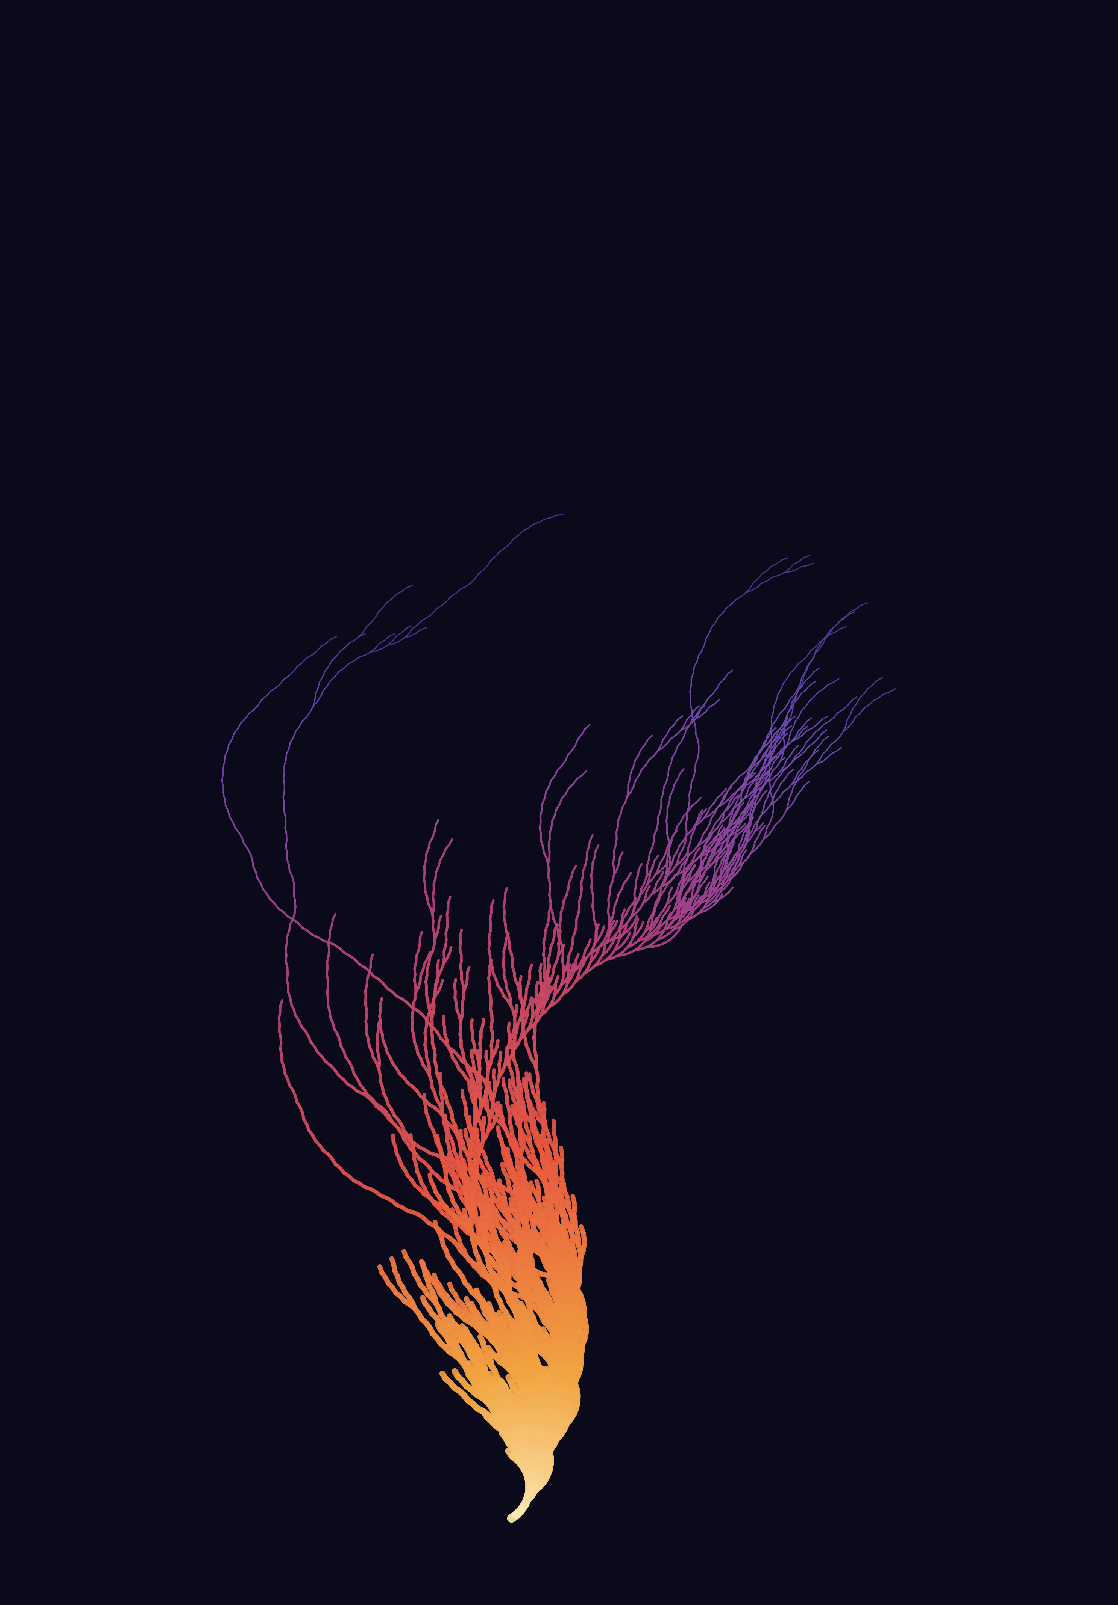
\includegraphics[width=7.25in]{art_cover}};
\end{scope}
\node[text=ink,align=center,text width=6.2in,anchor=north] at (\FrontC,9.3) {\fontsize{31}{37}\selectfont\scshape\mbox{On\hspace{0.32em}the\hspace{0.32em}Collatz\hspace{0.32em}Conjecture}};
\node[text=accent,align=center,text width=6.2in,anchor=north] at (\FrontC,8.35) {\fontsize{17}{21}\selectfont\itshape Martingales, Momentum and Continued Fractions};
\node[text=ink,align=center,text width=6.2in,anchor=north] at (\FrontC,7.75) {\fontsize{17}{21}\selectfont Nick Polson\qquad Vadim Sokolov};
% spine
\ifnum\InteriorPages>79
\node[text=ink,rotate=-90,anchor=center] at (\SpineC,6.6) {\fontsize{\SpineFont}{\SpineFont}\selectfont\scshape On the Collatz Conjecture};
\node[text=accent,rotate=-90,anchor=center] at (\SpineC,1.9) {\fontsize{\SpineFont}{\SpineFont}\selectfont\scshape Polson\enspace\textperiodcentered\enspace Sokolov};
\fi
% back
\node[text=ink,anchor=north west,text width=5.5in,align=left,inner sep=0] at (0.8,9.4) {%
\fontsize{11.25}{15.2}\selectfont\hyphenpenalty=10000\exhyphenpenalty=10000
{\color{accent}\fontsize{13.5}{17.5}\selectfont\itshape Take a positive integer. If it is even, halve it; if it is odd, triple it and add one. Repeat.\par}
\medskip
The Collatz conjecture says that every starting value eventually reaches $1$. It can be explained to a child in a minute and has resisted every attempt at proof since the 1930s. This book is about why.\par\smallskip
Reading the map as a random walk, an optimizer and a Diophantine problem, the authors split the conjecture into a divergence half, a law of large numbers for a single deterministic orbit, and a cycle half, a question about rational approximation of $\log_23$ that Diophantine information alone cannot finish. Along the way they prove that no Lyapunov function increasing in the number certifies descent over any fixed number of steps and that no finite residue sieve certifies descent for every integer, and they set out a computational path to the problem with its limits made precise.\par\smallskip
The arithmetic of the map also yields an algorithm. Switching MM, a first order method with momentum $\log_23-1$ applied on alternate steps, has an explicit linear rate at step $1/L$ on smooth strongly convex functions, and on quadratics with additive gradient noise, at steps up to $1/L$, its noise variance stays below $5/3$ times that of gradient descent for every momentum coefficient below one.\par\smallskip
With full proofs, open problems and code for every number, this is a book for probabilists, number theorists and optimizers alike.\par\bigskip
{\color{accent}\itshape Nick Polson} is the Robert Law, Jr.\ Professor of Econometrics and Statistics at the University of Chicago Booth School of Business. {\color{accent}\itshape Vadim Sokolov} is a faculty member in the Department of Systems Engineering and Operations Research at George Mason University.\par};
\node[anchor=south west,inner sep=0] at (0.8,0.6) {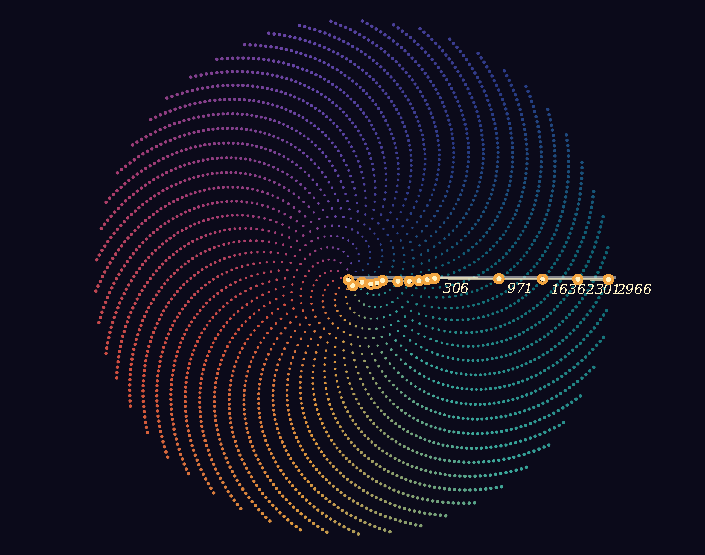
\includegraphics[width=1.9in]{art_part3}};
% barcode area, kept clear: KDP prints the barcode here
\fill[white] (4.875,0.375) rectangle (6.875,1.575);
\end{tikzpicture}
\end{document}
